\documentclass{beamer}
\usepackage{graphicx}


\usetheme{m}
\title{timeline: a Time Series Visualization Platform}
\date{May 3, 2016}
\author{Manuel Haid, Thomas Mauerhofer, and Matthias Wölbitsch}


\begin{document}
  \maketitle
  
  
  \begin{frame}{Motivation}   
    \textbf{time series}
    \begin{itemize}
     \item data sets in which time plays an essential role 
     \item i.e. data has a time dimension
     \item example: consumption of electricity
    \end{itemize}
    
    \textbf{visualization}
    \begin{itemize}
     \item usually the first step
     \item detect patterns, trends, \ldots
     \item important for later analysis and modeling 
    \end{itemize}
  \end{frame}
  
  
  \begin{frame}{Project}
    \textbf{time series visualization platform} 
    \hspace{\textheight}
    
    \textbf{back-end}
    \begin{itemize}
     \item Python
     \item data import (files, web APIs, sockets)
     \item data storage (pandas)
     \item visualization engine 
     \item RESTful API (flask)
    \end{itemize}
  \end{frame}
  
  
  \begin{frame}{Project}
    \textbf{front-end}
    \begin{itemize}
      \item HTML/JS
      \item visualization library 
      \begin{itemize}
        \item Cubism.js
        \item MetricsGraphics.js
        \item \ldots
      \end{itemize}
    \end{itemize}
    
    \textbf{visualizations}
    \begin{itemize}
     \item time series plots (filters, multiple time series)
     \item plot running average and standard deviation
     \item live updates for time series plots
     \item seasonal plots
     \item autocorrelation function (ACF) plots
     \item forecasting model evaluation plots
    \end{itemize}
  \end{frame}  

  
  \begin{frame}{Visualization examples}   
    \begin{columns}[c]
      \column{0.5\textwidth}  
      \begin{figure}
       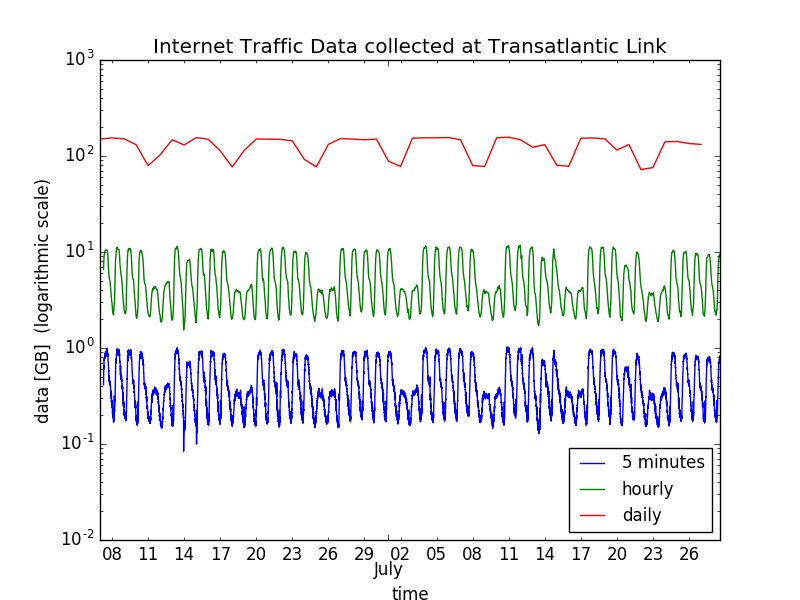
\includegraphics[width=1.0\textwidth]{images/timeplot.png}
       \caption{Exemplary time series plot of three different data sets.}
      \end{figure}

      \column{0.5\textwidth}
        \begin{figure}
         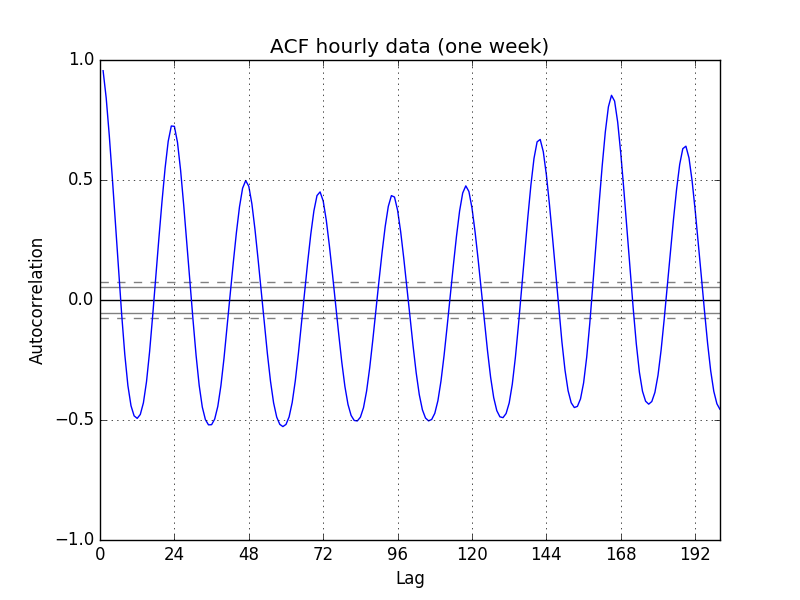
\includegraphics[width=1.0\textwidth]{images/acf.png}
         \caption{Example of a ACF plot that shows seasonal effects.}
        \end{figure}
    \end{columns}
  \end{frame}
  
  
  \plain{Questions?}
  
  
\end{document}